% Complemento C2: Transformaciones conformes
% Números y figuras PNG: apunte/scripts/c2_conformes.py (uv run python apunte/scripts/c2_conformes.py)
\capituloComplemento[2]{Transformaciones conformes}\label{cap:conformes}


\section{La idea}

Imaginá que pelás una naranja en pocos pedazos grandes y aplastás cada pedazo contra la mesa.
¿Se puede aplanar la cáscara sin rajarla ni estirarla en ningún lado?
No se puede, y la superficie de la Tierra tiene el mismo problema: ningún mapa plano la
representa sin deformar algo. Lo que sí podemos elegir es \emph{qué} se deforma.

Mirá el plano de un barrio de manzanas cuadradas.
¿Qué sería peor: que las esquinas dejaran de verse de \(90^\circ\), o que una cuadra lejos del centro del plano midiera, en el papel, un poco más que una cuadra del centro?
Para quien mide en el terreno lo primero es inaceptable, porque cada ángulo medido tiene que
poder dibujarse tal cual; lo segundo, en cambio, se corrige multiplicando por un número.

Tomá una foto de ese plano y estirala parejo en horizontal, un 50 por ciento.
¿Las calles siguen cortándose en ángulo recto? ¿Y una diagonal que cruza la manzana sigue formando \(45^\circ\) con la calle?
Las calles horizontales y verticales siguen perpendiculares, pero las diagonales se tuercen:
estirar parejo en una sola dirección no conserva los ángulos.

Pensá en una lupa que recorre el mapa.
¿Puede pasar que en cada lugar la lupa muestre una copia fiel del terreno, girada y agrandada, aunque el aumento cambie de un lugar a otro?
Ese es el mapa que buscamos: cerca de cada punto se comporta como una similaridad (un giro con
un cambio de tamaño, sección~\ref{sec:escalar}), y de un punto a otro cambia el tamaño.

Suponé que medís un lado de un kilómetro a cien kilómetros del centro de un mapa así.
¿Cuánto más largo sale dibujado? ¿Centímetros o metros?

Una transformación que conserva los ángulos chicos en cada punto se llama
\emph{transformación conforme}. Sirve porque deja dibujar cada ángulo del terreno sin
corregirlo; el precio es un \emph{factor de escala} \(k\), el número que dice cuántos metros
del mapa corresponden a un metro del terreno en cada lugar, y que hay que conocer. Al final
del complemento (sección~\ref{sec:conformes-aplicacion}) respondemos la última pregunta con
las coordenadas planas que se usan en la Argentina.

\subsection{Variable compleja y conformidad}

¿Cómo se escribe con números \enquote{girar y agrandar}? En el capítulo de rotaciones
(sección~\ref{sec:rot-complejos}) vimos que multiplicar por un número complejo
\(\rho e^{i\theta}\) gira en \(\theta\) y agranda en \(\rho\). Llamamos \(z\) al punto del
plano escrito como número complejo, \(w\) a su imagen y \(f\) a la regla que los une, \(w=f(z)\).
Una función compleja \(w=f(z)\) es derivable en sentido complejo cuando existe
\[
  f'(z)=\lim_{\Delta z\to0}
  \frac{f(z+\Delta z)-f(z)}{\Delta z}.
\]
Cuando \(f'(z)\neq0\), la transformación lineal local es multiplicación por el complejo
\(f'(z)\): una rotación combinada con un escalado uniforme. Por ello las funciones holomorfas
preservan ángulos localmente.
Dicho de otro modo, una transformación conforme es una similaridad distinta en cada punto
(sección~\ref{sec:mapa-transformaciones}).

\begin{idea}[Una conforme es una similaridad en cada punto, y deja de serlo en grande]
Cerca de cada punto \(p\), una transformación conforme actúa como la similaridad directa de
escala \(k(p)=\lvert f'(z)\rvert\) y giro \(\theta(p)=\arg f'(z)\): multiplicar por el
complejo \(f'(z)\). La escala y el giro son propios de cada punto, así que en una figura grande
ninguna similaridad sola la representa: las rectas se curvan, las paralelas dejan de serlo y
las áreas se multiplican por factores distintos en cada lugar. Es lo que registra la columna
Conforme del cuadro~\ref{tab:conserva}: ángulos y sentido de giro, sí; el resto, solo
localmente.
\end{idea}

La proyección estereográfica es un ejemplo central y conduce naturalmente al plano complejo
extendido
\[
  \widehat{\mathbb C}=\mathbb C\cup\{\infty\}.
\]
La relación entre rotaciones, multiplicación compleja y conformidad conecta el capítulo de
rotaciones (capítulo~\ref{cap:rotaciones}) con este.

\subsection{Proyecciones cartográficas}\label{sec:proyecciones}

¿Qué es, en general, un mapa? Una regla que a cada punto de la superficie de la Tierra le
asigna un punto del papel. Una proyección es una aplicación desde una superficie de referencia al plano:
\[
  P:S\longrightarrow\R^2.
\]
No puede conservar simultáneamente todas las propiedades métricas. Según la propiedad
priorizada se distingue:

\begin{center}
\begin{tabularx}{.92\textwidth}{>{\bfseries}l X X}
\toprule
Tipo & Conserva localmente & Ejemplos\\
\midrule
Conforme & ángulos & Mercator, Gauss--Krüger, UTM\\
Equivalente & áreas & Albers, Mollweide\\
Equidistante & ciertas distancias & azimutal equidistante\\
\bottomrule
\end{tabularx}
\end{center}

La derivada \(dP_p\) actúa entre planos tangentes. Sus valores singulares describen las
escalas principales de deformación; su determinante describe el cambio local de área.

\section{Construcciones, cuentas y ejemplos}

La cuenta va de punta a punta, del número complejo y el Jacobiano a la proyección del elipsoide, con la indicatriz de Tissot como figura. Es desarrollo complementario.

\subsection{Transformaciones conformes: del número complejo y el Jacobiano a la proyección del elipsoide}\label{sec:transformaciones-conformes}

{\small\linkAnimacion{06_conforme_tissot_mercator}{Animación: indicatriz de Tissot, equidistante vs. Mercator}\par}


\begin{atencion}[Desarrollo complementario]
Esta sección cierra el arco de la materia: el número complejo (sección~\ref{sec:rot-complejos}),
las similaridades (secciones~\ref{sec:escalar} y~\ref{cap:reflexiones}), la SVD
(sección~\ref{sec:svd}), el Jacobiano y la primera forma fundamental
(sección~\ref{sec:metrica}) son, vistos desde acá, cuatro maneras de decir lo mismo, y
el elipsoide (capítulo~\ref{cap:elipsoide}) es el escenario donde se aplican. Con ese
lenguaje se construyen las proyecciones del elipsoide al plano anunciadas al cierre de aquel capítulo, incluida la
transversa de Mercator.
\end{atencion}

\paragraph{El problema cartográfico.} En la sección~\ref{cap:curvatura} (capítulo~\ref{cap:curvatura}) calculamos que la
curvatura gaussiana del elipsoide es \(K=1/(MN)>0\) en todos los puntos; la del plano es
\(K=0\). El \emph{theorema egregium} de Gauss dice que \(K\) se puede calcular con la
primera forma fundamental sola (con \(E,F,G\) y sus derivadas), es decir, midiendo
longitudes \emph{dentro} de la superficie, sin salir a \(\R^3\). La consecuencia es
inmediata: si existiera una aplicación del elipsoide al plano que conservara todas las
longitudes (una isometría local), las dos superficies tendrían la misma \(K\), y
\(1/(MN)\neq0\). No existe. Toda carta, y todo sistema de coordenadas planas
(Gauss--Krüger en las fajas de POSGAR), deforma \emph{algo}: longitudes, áreas, ángulos o
una mezcla. Hecho geométrico: una cáscara de naranja no se aplana sin rajarse.

Entonces elegimos qué conservar. Un agrimensor no negocia el ángulo: los \(90^\circ\)
medidos en el terreno entre dos alineaciones tienen que cortarse a \(90^\circ\) en
el plano de la mensura, y la dirección de la tangente a una visual en el terreno tiene
que ser la del plano más una corrección que dependa del punto, no de la dirección (la
convergencia de meridianos; para un lado finito se suma además la corrección
arco-cuerda, que sí depende de la dirección y del largo). Eso es una
\emph{transformación conforme}: en cada punto conserva los ángulos entre curvas, con su
orientación (no refleja). Lo que sí cambia de punto a punto es la escala, y la pagamos con
un factor \(k(P)\) que hay que conocer (la \enquote{escala de la proyección}).

\paragraph{Qué es una transformación en un punto.} Una aplicación \(P\mapsto P'\) entre
superficies (o entre planos) es, cerca de cada punto, su jacobiana \(J(P)\): la matriz
\(2\times2\) que lleva un pasito \((du,dv)\) del terreno al pasito correspondiente del mapa
(sección~\ref{sec:metrica}). Para que \enquote{conservar ángulos} tenga sentido métrico, medimos
los pasitos del terreno con la primera forma del terreno y los del mapa con la del mapa; en
lo que sigue suponemos que trabajamos en bases ortonormales de los dos planos tangentes
(sobre el elipsoide, \(r_\varphi/M\) y \(r_\lambda/(N\cos\varphi)\); en el plano, los
versores), de modo que \(J\) es una matriz real \(2\times2\) común y corriente y la
pregunta \enquote{¿conserva ángulos?} es la de las similaridades (sección~\ref{sec:escalar}).

\begin{resultado}[Las cuatro caras de una transformación conforme]
Sea \(J=J(P)\) la jacobiana en un punto, con \(\det J>0\) (invertible y sin reflejar:
conserva la orientación). Son equivalentes:
\begin{enumerate}[label=(\roman*)]
  \item \textbf{Similaridad directa.} \(J=\rho\,R(\theta)\) con \(\rho>0\): una rotación
  seguida de una homotecia, la similaridad directa con punto fijo
  (sección~\ref{sec:escalar}).
  \item \textbf{Valores singulares iguales.} \(\sigma_1=\sigma_2=k\) en la SVD de \(J\)
  (sección~\ref{sec:svd}): la indicatriz de Tissot (la imagen de la circunferencia unidad
  del terreno) es una circunferencia de radio \(k\), no una elipse.
  \item \textbf{Métrica proporcional.} \(J^TJ=k^2I\): en la primera forma inducida,
  \(F=0\) y \(E=G=k^2\), es decir \(ds^2_{\text{mapa}}=k^2\,ds^2_{\text{terreno}}\).
  \item \textbf{Número complejo.} \(J=\begin{pmatrix}a&-b\\b&a\end{pmatrix}\), la matriz
  de multiplicar por \(a+ib\) (sección~\ref{sec:rot-complejos}). Si la transformación
  \((u,v)\mapsto(x,y)\) tiene derivadas parciales continuas (\(C^1\)), esto son las ecuaciones de Cauchy--Riemann
  \[
    x_u=y_v,\qquad x_v=-y_u ,
  \]
  y \(J\) es multiplicar por \(f'(z)=x_u+i\,y_u\), con \(z=u+iv\) y \(f=x+iy\): toda
  función analítica con \(f'(z)\neq0\) es conforme, y recíprocamente toda aplicación \(C^1\) que cumple Cauchy--Riemann con derivada no nula es analítica y conforme.
\end{enumerate}
En todas, \(k=\rho=|f'(z)|=\sqrt{\det J}\) es la escala local y \(\theta=\arg f'(z)\) la
rotación local (la \enquote{convergencia de meridianos} en las proyecciones).
\end{resultado}

\emph{Demostración.} Son tres equivalencias con el centro en (i).

(i)\(\Leftrightarrow\)(iv), por la forma de las matrices. Una rotación por homotecia es
\[
  \rho\,R(\theta)=\begin{pmatrix}\rho\cos\theta&-\rho\sin\theta\\ \rho\sin\theta&\rho\cos\theta\end{pmatrix}
  =\begin{pmatrix}a&-b\\b&a\end{pmatrix}\quad\text{con } a=\rho\cos\theta,\ b=\rho\sin\theta ,
\]
y al revés: toda matriz \(\begin{pmatrix}a&-b\\b&a\end{pmatrix}\) con \((a,b)\neq(0,0)\)
se escribe así tomando \(\rho=\sqrt{a^2+b^2}\) y \(\theta=\operatorname{atan2}(b,a)\). Es
exactamente la identificación \(\rho e^{i\theta}\leftrightarrow\rho R(\theta)\) de los números
complejos (sección~\ref{sec:rot-complejos}): la matriz de la izquierda tiene dos parámetros, no cuatro. Leer \(a=x_u\),
\(b=y_u\) y comparar con la jacobiana general
\(\begin{pmatrix}x_u&x_v\\y_u&y_v\end{pmatrix}\) da Cauchy--Riemann.

(i)\(\Leftrightarrow\)(ii), por la SVD. Si \(J=U\Sigma V^T\) con \(\Sigma=kI\), entonces
\(J=k\,UV^T\), y \(UV^T\) es ortogonal (producto de ortogonales) con
\(\det(UV^T)=\det J/k^2\). Acá usamos la hipótesis \(\det J>0\): ese determinante es
\(+1\), así que \(UV^T\) es una rotación y \(J=k\,R(\theta)\). Sin la hipótesis, \(UV^T\)
podría ser una reflexión: \(J=\operatorname{diag}(1,-1)\) tiene \(\sigma_1=\sigma_2=1\) y no
es una similaridad directa. Al revés, si
\(J=\rho R(\theta)\), su SVD es \(U=R(\theta)\), \(\Sigma=\rho I\), \(V=I\), y los dos
valores singulares valen \(\rho\). Geométricamente: la circunferencia unidad va a una
elipse de semiejes \(\sigma_1,\sigma_2\); la elipse es circunferencia si y solo si los
semiejes son iguales.

(i)\(\Leftrightarrow\)(iii), por el producto \(J^TJ\). La primera forma inducida es
\(ds^2_{\text{mapa}}=(du\ dv)\,J^TJ\,(du\ dv)^T\), de modo que \(E,F,G\) son las
entradas de \(J^TJ\). Si \(J=\rho R\), \(J^TJ=\rho^2R^TR=\rho^2I\): \(F=0\) y
\(E=G=\rho^2\). Al revés, si \(J^TJ=k^2I\), la matriz \(J/k\) cumple \((J/k)^T(J/k)=I\),
es ortogonal; por la hipótesis \(\det J>0\) es una rotación y \(J=k\,R(\theta)\). (Con
\(\det J<0\) sería una reflexión por una homotecia: conserva el tamaño de los ángulos pero
invierte la orientación, una similaridad inversa; por eso la hipótesis va en el enunciado:
sin ella (ii) y (iii) no implican (i). Las proyecciones cartográficas se toman directas.)
\(\square\)

\begin{ejemplo}[La lupa de \(w=z^2\) en \(1+i\)]\label{ej:conf-z2}
¿Qué hace \(w=z^2\) cerca del punto \(z_0=1+i\)? Su derivada es \(f'(z)=2z\), así que
\(f'(z_0)=2+2i\): la lupa en ese punto agranda \(k=\lvert2+2i\rvert=2\sqrt2\approx2{,}8284\)
veces y gira \(\theta=\arg(2+2i)=45^\circ\). Lo comprobamos con dos pasitos perpendiculares
de largo \(h\), uno hacia la derecha (\(z_0+h\)) y otro hacia arriba (\(z_0+ih\)). Con
\(h=0{,}1\), las imágenes se corren
\[
  (z_0+h)^2-z_0^2=2z_0h+h^2=0{,}21+0{,}2\,i,\qquad
  (z_0+ih)^2-z_0^2=2z_0ih-h^2=-0{,}21+0{,}2\,i ,
\]
que forman un ángulo de \(92{,}79^\circ\) y miden \(2{,}9000\,h\) cada una. Con \(h=0{,}01\) el
ángulo baja a \(90{,}29^\circ\) y el largo a \(2{,}8355\,h\). Cuanto más chico el pasito, más se
acercan al ángulo recto y al aumento \(2{,}8284\) que predice \(f'(z_0)\): la conformidad es
una propiedad del límite, y el término \(h^2\) es lo que la cuadrícula grande ve curvado
(figura~\ref{fig:conf-cuadricula}, centro).
\end{ejemplo}

\begin{figure}[htbp]
\centering
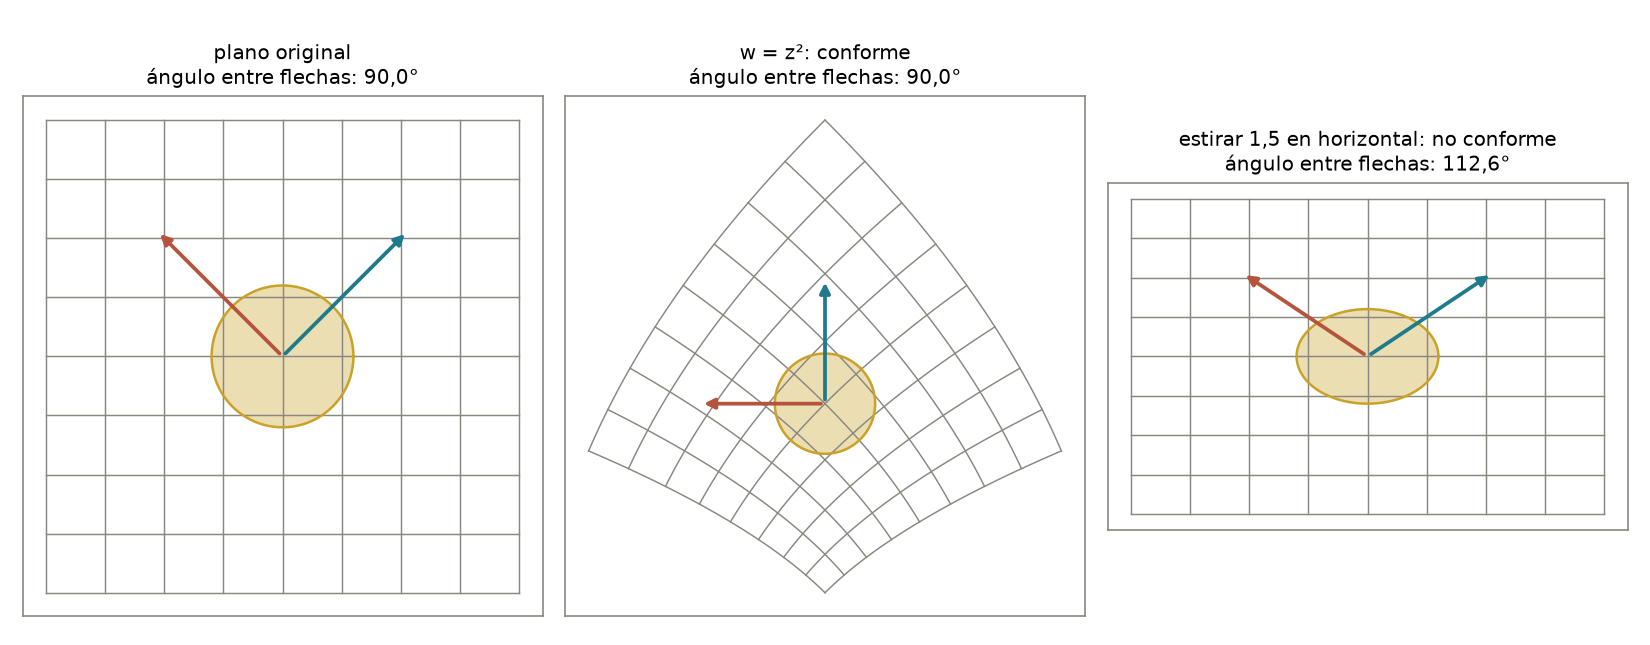
\includegraphics[width=\linewidth]{figuras/conformes/conf_cuadricula.png}
\caption{Una cuadrícula chica alrededor de \(1+i\) (izquierda), su imagen por \(w=z^2\)
(centro) y su imagen por el estiramiento \(\operatorname{diag}(1{,}5;\ 1)\) (derecha). Las
flechas son dos direcciones a \(90^\circ\) y el círculo, uno chico centrado en el punto. En
el centro, flechas y círculo están dibujados con la lupa \(f'(1+i)\): las líneas de la
cuadrícula se curvan pero se siguen cortando a \(90^\circ\), y el círculo sigue siendo círculo.
A la derecha las flechas pasan a formar \(112{,}6^\circ\) y el círculo se vuelve elipse.
Generada con \texttt{apunte/scripts/c2\_conformes.py}.}
\label{fig:conf-cuadricula}
\end{figure}

\paragraph{El conjugado complejo: transponer es reflejar.}\phantomsection\label{sec:conjugado-complejo}
Para un número complejo \(z=a+ib\) se escribe
\(J(z)=\left(\begin{smallmatrix}a&-b\\b&a\end{smallmatrix}\right)\), la matriz de (iv): la de
multiplicar por \(z\), que es la jacobiana de \(\zeta\mapsto z\zeta\). El conjugado
\(\bar z=a-ib\) tiene una lectura matricial directa.

\begin{proposicion}[El conjugado complejo como transpuesta y como reflexión]\label{prop:conjugado-complejo}
Sea \(z=a+ib\) y \(S=\operatorname{diag}(1,-1)\). Entonces
\[
  J(\bar z)=J(z)^T=S\,J(z)\,S
  \qquad\text{y}\qquad
  \lvert z\rvert^2=\det J(z).
\]
\end{proposicion}

\begin{demostracion}
Es una cuenta. Por definición, \(J(\bar z)=J(a+i(-b))=\left(\begin{smallmatrix}a&b\\-b&a\end{smallmatrix}\right)\),
que es \(J(z)^T\). Multiplicar a izquierda por \(S\) cambia el signo de la segunda fila y
multiplicar a derecha por \(S\) cambia el signo de la segunda columna:
\[
  S\,J(z)\,S=\begin{pmatrix}1&0\\0&-1\end{pmatrix}\begin{pmatrix}a&-b\\b&a\end{pmatrix}
  \begin{pmatrix}1&0\\0&-1\end{pmatrix}
  =\begin{pmatrix}a&-b\\-b&-a\end{pmatrix}\begin{pmatrix}1&0\\0&-1\end{pmatrix}
  =\begin{pmatrix}a&b\\-b&a\end{pmatrix}=J(\bar z).
\]
Por último, \(\det J(z)=a\cdot a-(-b)\cdot b=a^2+b^2=z\bar z=\lvert z\rvert^2\). Por ejemplo,
con \(z=3+4i\): \(J(z)^T=\left(\begin{smallmatrix}3&4\\-4&3\end{smallmatrix}\right)=J(3-4i)\)
y \(\det J(z)=9+16=25=\lvert3+4i\rvert^2\).
\end{demostracion}

Tres lecturas. Primera: \emph{transponer la matriz de \(z\) es conjugar \(z\)}; de ahí que
\(J(z)J(z)^T=J(z\bar z)=\lvert z\rvert^2I\), es decir, \(J(z)/\lvert z\rvert\) es ortogonal, la
rotación \(R(\theta)\) de (i). Segunda: la aplicación \(z\mapsto\bar z\), \((a,b)\mapsto(a,-b)\),
tiene matriz \(S\): es la \emph{reflexión en el eje real}. No es multiplicar por ningún
complejo (\(S\) no tiene la forma \(J(w)\) y \(\det S=-1\)); como \(\arg\bar z=-\arg z\),
invierte el sentido de giro. \(S\) es ortogonal, así que cumple (iii) con \(k=1\) y conserva
el tamaño de los ángulos, pero con \(\det S<0\): es \emph{anticonforme}, el caso que la
hipótesis \(\det J>0\) deja afuera en el resultado anterior. Es lo que registra la columna
Reflexión del cuadro~\ref{tab:conserva}: distancias y ángulos, sí; sentido de giro, no.
Tercera: como \(S^{-1}=S\), la igualdad \(J(\bar z)=S^{-1}J(z)\,S\) dice que \(J(\bar z)\) es
\emph{conjugada} de \(J(z)\) por \(S\) en el sentido de la sección~\ref{sec:conjugacion}:
multiplicar por \(\bar z\) es reflejar, multiplicar por \(z\) y volver a reflejar,
\(\bar z\,w=\overline{z\,\bar w}\). La palabra \enquote{conjugado} aparece así con dos sentidos que
acá coinciden; el glosario de la sección~\ref{sec:glosario} los separa.

\begin{atencion}[¿Sobre qué Jacobiano pedimos \(J^TJ=k^2I\)? Coordenadas \((\varphi,\lambda)\) vs.\ metros en el plano tangente]
\emph{En coordenadas.} Si derivamos la carta \(\Phi(\varphi,\lambda)=(x,y)\) respecto de las
coordenadas geodésicas en radianes, obtenemos el Jacobiano de coordenadas
\(J_{\varphi,\lambda}=\partial(x,y)/\partial(\varphi,\lambda)\). Pero \((\varphi,\lambda)\) no
están en metros ni son isótropas: el elipsoide tiene la primera forma fundamental
\(\mathbf G=\operatorname{diag}(M^2,\,N^2\cos^2\varphi)\) (la matriz de la primera forma, con
\(E=M^2\), \(F=0\), \(G=N^2\cos^2\varphi\)). La condición exacta de conformidad es
entonces
\[
  J_{\varphi,\lambda}^T\,J_{\varphi,\lambda}=k(\varphi,\lambda)^2\,\mathbf G
  =k^2\begin{pmatrix}M^2&0\\0&N^2\cos^2\varphi\end{pmatrix}.
\]
Pedir \(J_{\varphi,\lambda}^TJ_{\varphi,\lambda}=k^2I\) directo sobre \((\varphi,\lambda)\)
sería el error de la hoja cuadriculada de la sección~0: tratar radianes de latitud y de
longitud como si midieran lo mismo.

\emph{En metros.} Cuando pasamos a la base ortonormal en metros del plano tangente
(\(ds_{\text{mer}}=M\,d\varphi\), \(ds_{\text{par}}=N\cos\varphi\,d\lambda\)), el Jacobiano
físico es
\[
  \tilde J=J_{\varphi,\lambda}\,\mathbf G^{-1/2}
  =J_{\varphi,\lambda}\,\operatorname{diag}\!\Bigl(\frac1M,\,\frac1{N\cos\varphi}\Bigr),
\]
y recién ahí la condición toma la forma euclídea \(\tilde J^T\tilde J=k^2I\) (con
\(\det\tilde J>0\) para conservar la orientación). El \(\tilde J\) es el que mira la unidad
(la cara~(i) de arriba), y \(h\) y \(k\) son sus escalas en meridiano y paralelo.
\end{atencion}

\paragraph{Conforme es una propiedad local.} Una proyección conforme conserva exactamente
el ángulo en el punto donde se cortan dos curvas y lleva circulitos infinitesimales en
circulitos. Pero el factor de escala \(k(P)\) varía con la posición, así que las figuras
extensas no mantienen ni su área ni su forma global (Groenlandia en Mercator parece del
tamaño de África). Por eso, en la Argentina, POSGAR divide el país en 7 fajas de
Gauss--Krüger de \(3^\circ\) de ancho: no para \enquote{mantener la conformidad} (Gauss--Krüger
ya es conforme a cualquier distancia del meridiano central), sino para acotar la
deformación lineal \(k-1\approx\tfrac12\,\Delta\lambda^2\cos^2\varphi\) (con \(\Delta\lambda\)
en radianes) por debajo de unos \(2{,}3\times10^{-4}\), es decir \(23\) cm/km, en el borde de la
faja (\(\Delta\lambda=1{,}5^\circ\), es decir longitud \(-58{,}5^\circ\)) a la latitud de Buenos Aires
(\(\varphi=-34{,}6^\circ\)). La cifra se calcula sobre el elipsoide GRS80 (\(a=6\,378\,137\) m,
\(1/f=298{,}257222101\); POSGAR 2007, faja 5 de meridiano central \(-60^\circ\), \(k_0=1\)): la aproximación da \(2{,}32\times10^{-4}\) y el
factor de escala exacto, \(2{,}33\times10^{-4}\). Los \(34\) cm/km corresponden al
ecuador (\(\cos\varphi=1\), \(3{,}45\times10^{-4}\) exacto), que es el peor caso de la
faja.

\paragraph{Por qué (iii) es \enquote{conservar ángulos}.} El ángulo entre dos pasitos \(p,q\)
del terreno se calcula con el producto interno, \(\cos\alpha=p\cdot q/(\|p\|\|q\|)\). En el
mapa los pasitos son \(Jp\) y \(Jq\), y \((Jp)\cdot(Jq)=p^T(J^TJ)q=k^2\,p\cdot q\): el
numerador se multiplica por \(k^2\), cada norma por \(k\), y el coseno no cambia. Es el
mismo argumento del capítulo de rotaciones (el producto interno es invariante por rotaciones) con una
homotecia más. Y es lo único que lo logra: si \(J^TJ\) no fuera múltiplo de la identidad,
sus dos autovectores (las direcciones \(v_1,v_2\) de la SVD) se estirarían distinto y
alguna dirección intermedia giraría respecto de las otras.

\paragraph{Cuánto se deforma un ángulo cuando no es conforme.} Con la SVD podemos
medirlo. En las bases \(v_1,v_2\) y \(u_1,u_2\) la jacobiana es \(\operatorname{diag}(\sigma_1,\sigma_2)\),
\(\sigma_1\ge\sigma_2>0\). La dirección de ángulo \(\alpha\) del terreno,
\((\cos\alpha,\sin\alpha)\), va a \((\sigma_1\cos\alpha,\sigma_2\sin\alpha)\), de ángulo
\(\alpha'\) con \(\tan\alpha'=r\tan\alpha\), \(r=\sigma_2/\sigma_1\le1\). El giro de esa
dirección es \(\delta=\alpha-\alpha'\), con
\[
  \tan\delta=\frac{\tan\alpha-\tan\alpha'}{1+\tan\alpha\tan\alpha'}
  =\frac{(1-r)\,t}{1+r\,t^2},\qquad t=\tan\alpha .
\]
Derivando en \(t\) y anulando, \(1+rt^2-2rt^2=0\), o sea \(t^2=1/r\): el giro es máximo
en la dirección con \(\tan\alpha=\sqrt{\sigma_1/\sigma_2}\), y ahí
\(\tan\alpha'=\sqrt{\sigma_2/\sigma_1}=1/\tan\alpha\), de modo que \(\alpha+\alpha'=90^\circ\):
la dirección y su imagen son simétricas respecto de la diagonal de la elipse. En ese
máximo \(\tan\delta=(1-r)/(2\sqrt r)\), y pasando a seno
(\(\sin\delta=\tan\delta/\sqrt{1+\tan^2\delta}\), con \((1-r)^2+4r=(1+r)^2\)):
\[
  \sin\delta_{\max}=\frac{1-r}{1+r}=\frac{\sigma_1-\sigma_2}{\sigma_1+\sigma_2}.
\]
La dirección simétrica, de ángulo \(-\alpha\), gira lo mismo en sentido contrario, así
que el ángulo \(2\alpha\) entre ambas es el que más cambia, y cambia en
\[
  \boxed{\ \omega=2\arcsin\frac{\sigma_1-\sigma_2}{\sigma_1+\sigma_2}\ }
\]
(deformación angular máxima de Tissot). Control: \(\omega=0\) si y solo si
\(\sigma_1=\sigma_2\), que es (ii). Con \(r=1/2\), \(\omega=38{,}94^\circ\), lo mismo
que da maximizar numéricamente \(2(\alpha-\alpha')\).

\begin{ejemplo}[Una foto estirada parejo no es conforme]\label{ej:conf-foto}
Estirar una foto un 50 por ciento en horizontal es aplicarle \(J=\operatorname{diag}(1{,}5;\ 1)\),
la misma matriz en todos los puntos. Las direcciones horizontal y vertical son las de la SVD
y siguen perpendiculares. La diagonal de \(45^\circ\), \((1,1)\), va a \((1{,}5;\ 1)\), de
ángulo \(\arctan(1/1{,}5)=33{,}69^\circ\), y la de \(135^\circ\) va a la simétrica: el ángulo
recto entre las dos diagonales se dibuja de \(112{,}62^\circ\). Con \(r=1/1{,}5\), la fórmula de
Tissot da \(\omega=2\arcsin\frac{0{,}5}{2{,}5}=23{,}07^\circ\), algo más que los
\(22{,}62^\circ\) de las diagonales: el máximo ocurre en la dirección
\(\alpha=\arctan\sqrt{1{,}5}=50{,}77^\circ\), que va a \(39{,}23^\circ\) (suman \(90^\circ\), como
predice la cuenta de arriba). Ningún estiramiento en una sola dirección es conforme, por más
parejo que sea; una conforme puede cambiar el tamaño de un lugar a otro, pero en cada lugar
estira igual en todas las direcciones (figura~\ref{fig:conf-cuadricula}, derecha).
\end{ejemplo}

\unidadInteractiva{15_transformaciones_conformes}{Transformaciones conformes}{Explorá: en «caso precargado» elegí el mapa complejo en el plano. Con la función compleja \(w=z^2\), comprobá que el círculo sigue siendo círculo y que el ángulo entre las dos visuales no cambia al mover «rumbo α (°) de la primera visual». Después pasá a la función \(w=z+\alpha\bar z\), mové el deslizador de \(\alpha\) desde \(0\) y mirá cómo el círculo se vuelve elipse, como la foto estirada del ejemplo~\ref{ej:conf-foto}.}

\subsection{Aplicación topográfica: el factor de escala de Gauss-Krüger en la faja 5}\label{sec:conformes-aplicacion}

Contada en llano, la situación es esta. Quien mide un terreno no anota latitudes y longitudes
sino coordenadas planas en metros, \((E,N)\): cuántos metros al este y cuántos al norte de un
origen. Para pasar de la superficie curva al plano, la Argentina usa una proyección conforme
(la de Gauss-Krüger, la transversa de Mercator de la sección~\ref{sec:conformes-elipsoide})
aplicada por franjas angostas: cada \emph{faja} es una franja de \(3^\circ\) de longitud de
ancho con su propio meridiano central, y el marco oficial de coordenadas del país, POSGAR 2007,
numera esas franjas del 1 al 7. Por ser conforme, un ángulo recto medido en el terreno se
dibuja recto en el plano en cualquier lugar de la franja. Lo que se paga es la escala: sobre
el meridiano central un kilómetro del terreno es un kilómetro del plano, y a medida que nos
alejamos hacia el este o el oeste el plano estira un poco. ¿Cuánto? Lo calculamos en la
franja 5, la de meridiano central \(\lambda_0=-60^\circ\), que es la de la ciudad de Buenos
Aires.

\paragraph{Qué pedimos y a quién.} Usamos la biblioteca \texttt{pyproj} (versión \texttt{3.8.0}, sobre
PROJ \texttt{9.8.1}), que implementa las proyecciones oficiales. Le pedimos el sistema de coordenadas
de código EPSG:5347 (\enquote{POSGAR 2007 / Argentina 5}), que trae meridiano central
\(-60^\circ\), factor de escala \(1\) sobre él y \(5\,500\,000\) m sumados al este para que no
haya coordenadas negativas (por eso importa la diferencia \(\Delta E\), el este menos esos
\(5\,500\,000\) m, y no el número completo). Tomamos cuatro puntos sintéticos, todos a la latitud
de ejemplo \(\varphi=-34{,}6^\circ\), a \(\Delta E=0\), \(50\), \(100\) y \(150\) km al este del
meridiano central. Para cada uno, el script busca la longitud que da ese \(\Delta E\) y le pide
a la función \texttt{get\_factors} de \texttt{pyproj.Proj} la escala a lo largo del meridiano,
la escala a lo largo del paralelo y la convergencia de meridianos (el ángulo entre el norte
del plano y el meridiano del lugar). PROJ declara para ese código el elipsoide WGS84, que para
estas cifras es el mismo que GRS80 (capítulo~\ref{cap:elipsoide}).

\paragraph{La cuenta de bolsillo.} Junto al valor exacto ponemos la aproximación
\[
  k\approx1+\frac{(\Delta E)^2}{2R^2},
\]
con \(R\) el radio medio \(R_1=(2a+b)/3=6\,371\,008{,}771\) m del capítulo del elipsoide
(figura~\ref{fig:elip-radios}). De dónde sale lo mostramos en la
sección~\ref{sec:conformes-escala-serie}; en una esfera de radio \(R\) es la escala de la
transversa de Mercator hasta segundo orden.

\begin{ejemplo}[El factor de escala a \(0\), \(50\), \(100\) y \(150\) km del meridiano central]\label{ej:conf-faja5}
Valores de \texttt{pyproj} y de la aproximación con \(R_1\), en \(\varphi=-34{,}6^\circ\); la
columna \enquote{diferencia} es exacto menos aproximado.

{\small
\begin{center}
\begin{tabular}{r r r r r r r}
\toprule
\(\Delta E\) (km) & \(\lambda\) & \(k\) (\texttt{pyproj}) & \(k-1\) (cm/km) & aprox.\ (cm/km) & diferencia (mm/km) & convergencia\\
\midrule
0 & \(-60^\circ\) & 1{,}00000000 & 0{,}00 & 0{,}00 & 0{,}000 & \(0^\circ\)\\
50 & \(-59{,}4549^\circ\) & 1{,}00003080 & 3{,}08 & 3{,}08 & 0{,}005 & \(-0{,}3095^\circ\)\\
100 & \(-58{,}9099^\circ\) & 1{,}00012321 & 12{,}32 & 12{,}32 & 0{,}022 & \(-0{,}6191^\circ\)\\
150 & \(-58{,}3648^\circ\) & 1{,}00027722 & 27{,}72 & 27{,}72 & 0{,}056 & \(-0{,}9287^\circ\)\\
\bottomrule
\end{tabular}
\end{center}
}

En los cuatro puntos la escala a lo largo del meridiano y la escala a lo largo del paralelo
que devuelve \texttt{pyproj} coinciden (difieren en menos de \(10^{-9}\), el error de la
derivada numérica): es la cara (ii) de las transformaciones conformes, \(\sigma_1=\sigma_2\),
leída en una biblioteca oficial.
\end{ejemplo}

\paragraph{Lectura.} Primero, el estiramiento crece con el cuadrado de la distancia: al
duplicar \(\Delta E\) de \(50\) a \(100\) km, \(k-1\) se multiplica por cuatro, de \(3{,}08\) a
\(12{,}32\) cm por kilómetro (figura~\ref{fig:conf-k}). Segundo, el último punto está fuera de
la franja: en esta latitud el borde, \(\lambda=-58{,}5^\circ\), queda a \(137{,}6\) km del
meridiano central, y ahí \(k-1\) llega a \(2{,}33\times10^{-4}\), los \(23\) cm/km del párrafo
\enquote{Conforme es una propiedad local}. Partir el país en franjas angostas es lo que mantiene
el estiramiento por debajo de eso. Tercero, la cuenta de bolsillo alcanza de sobra: con
\(R_1\) se equivoca en \(0{,}056\) mm por kilómetro a \(150\) km, y con el radio
\(\sqrt{MN}=6\,370\,503{,}553\) m de esa latitud, en \(0{,}012\) mm por kilómetro
(figura~\ref{fig:conf-exacta-aprox}). Cuarto, como las áreas se multiplican por \(k^2\), a
\(150\) km del meridiano central una hectárea del terreno ocupa en el plano
\(10\,000+5{,}55\) m\(^2\). Por último, la convergencia de meridianos crece casi en proporción a la diferencia de
longitud (ejercicio~\ref{ex:conf-convergencia}).

\begin{figure}[htbp]
\centering
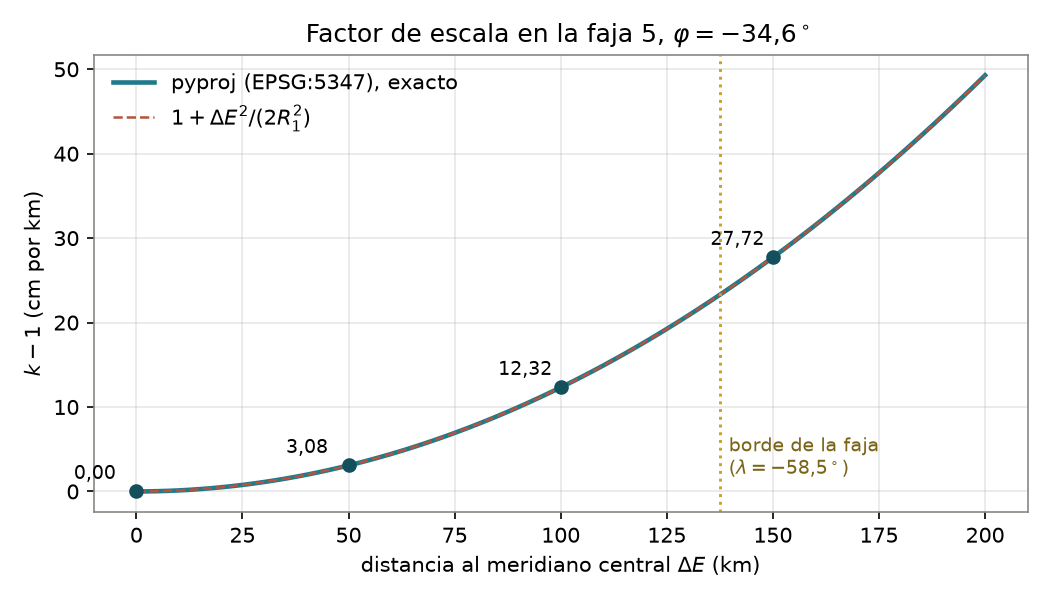
\includegraphics[width=.8\linewidth]{figuras/conformes/conf_k_DeltaE.png}
\caption{Estiramiento \(k-1\), en centímetros por kilómetro, en función de la distancia
\(\Delta E\) al meridiano central de la franja 5, a la latitud de ejemplo
\(\varphi=-34{,}6^\circ\). Línea llena: \texttt{pyproj} \texttt{3.8.0} con EPSG:5347; trazos: la
aproximación \(1+\Delta E^2/(2R_1^2)\), que a esta escala no se distingue. Los puntos son los del
ejemplo~\ref{ej:conf-faja5} y la línea punteada, el borde de la franja.}
\label{fig:conf-k}
\end{figure}

\begin{figure}[htbp]
\centering
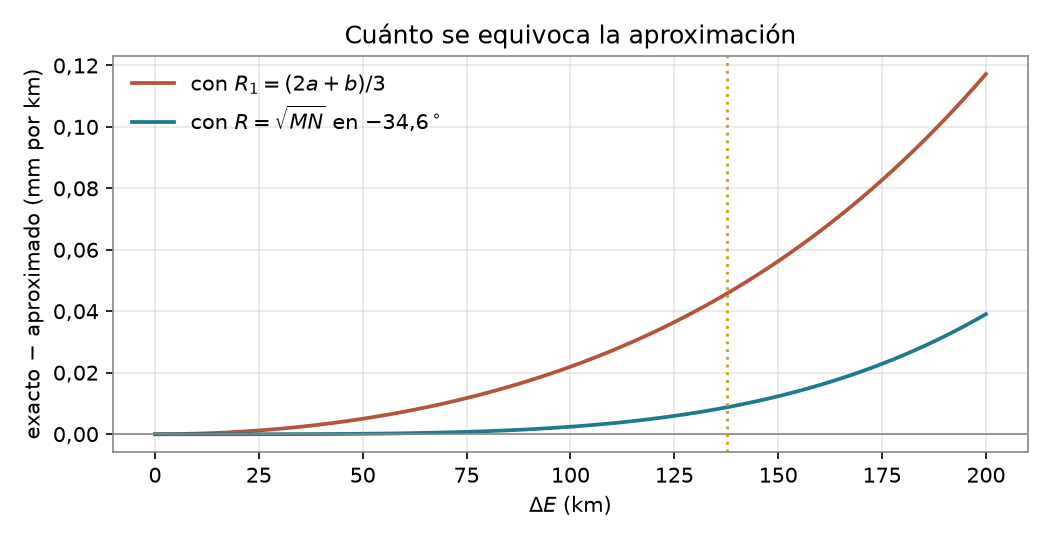
\includegraphics[width=.8\linewidth]{figuras/conformes/conf_exacta_aprox.png}
\caption{Diferencia entre la escala exacta (\texttt{pyproj}) y la aproximada, en milímetros por
kilómetro, con el radio medio \(R_1\) y con el radio \(\sqrt{MN}\) de la latitud de ejemplo.
Dentro de la franja (a la izquierda de la línea punteada) las dos quedan por debajo de
\(0{,}05\) mm por kilómetro; \(\sqrt{MN}\) es mejor por la razón que da la
sección~\ref{sec:conformes-escala-serie}.}
\label{fig:conf-exacta-aprox}
\end{figure}

En la práctica, lo que esto dice es que una distancia medida en el terreno no se copia tal
cual al plano: se multiplica por el \(k\) del lugar. Un lado de un kilómetro a \(100\) km del
meridiano central se dibuja \(12{,}3\) cm más largo; los ángulos, en cambio, pasan sin
corrección de escala. La dependencia de los radios con la latitud se puede explorar en la
unidad del elipsoide.

{\small\linkUnidad{13_elipsoide}{Simulación interactiva: geometría del elipsoide (los radios \(M\), \(N\) y \(\sqrt{MN}\) según la latitud)}\par}

\section{En profundidad}

Con el lenguaje ya armado, estudiamos las proyecciones principales del elipsoide al plano y las leemos según qué propiedad geométrica conservan.

\subsection{Las proyecciones del elipsoide con este lenguaje}\label{sec:conformes-elipsoide}

\paragraph{Cinco maneras de llevar el elipsoide al plano.} Apoyándonos en la métrica y el arco de meridiano del capítulo~\ref{cap:elipsoide}, recorremos cinco construcciones clásicas
integrando una condición cada vez y leyéndolas con las cuatro caras. Sobre el
elipsoide, con la base \((\varphi,\lambda)\),
\[
  ds^2=M^2\,d\varphi^2+N^2\cos^2\varphi\,d\lambda^2 :
\]
\(F=0\), la grilla de meridianos y paralelos es ortogonal, pero un paso \(d\varphi=d\lambda\)
no es un cuadradito: mide \(M\,d\varphi\) hacia el norte y \(N\cos\varphi\,d\lambda\) hacia
el este. En una proyección cilíndrica \(x=a\lambda\), \(y=y(\varphi)\), la jacobiana en las
bases ortonormales del terreno y del plano es diagonal,
\[
  J=\operatorname{diag}(h,k),\qquad
  h=\frac{dy/d\varphi}{M}\ \ (\text{meridiano}),\qquad
  k=\frac{dx/d\lambda}{N\cos\varphi}=\frac{a}{N\cos\varphi}\ \ (\text{paralelo}),
\]
así que \(\{\sigma_1,\sigma_2\}=\{h,k\}\) y cada condición es una ecuación en \(h\) y \(k\).
\begin{enumerate}[label=(\alph*)]
  \item \textbf{Mercator: conforme.} Cara (ii), \(h=k\):
  \[
    \frac{dy}{d\varphi}=\frac{a\,M}{N\cos\varphi}
    \quad\Longrightarrow\quad
    y=a\,q(\varphi),\qquad
    q(\varphi)=\int_0^\varphi\frac{M}{N\cos u}\,du ,
  \]
  la \emph{latitud isométrica}. La integral sale con una identidad: como
  \(M/N=(1-e^2)/(1-e^2\sin^2\varphi)\),
  \[
    \frac{M}{N\cos\varphi}=\frac{1-e^2}{(1-e^2\sin^2\varphi)\cos\varphi}
    =\frac1{\cos\varphi}-\frac{e^2\cos\varphi}{1-e^2\sin^2\varphi}
  \]
  (se verifica poniendo a común denominador: \(1-e^2\sin^2\varphi-e^2\cos^2\varphi=1-e^2\)).
  El primer término integra \(\ln\tan(\pi/4+\varphi/2)\), el de Mercator esférico. En el
  segundo, con \(t=\sin\varphi\), queda \(e^2\int dt/(1-e^2t^2)\), y las fracciones simples
  \(\frac1{1-e^2t^2}=\frac12\bigl(\frac1{1+et}+\frac1{1-et}\bigr)\) dan
  \(\frac e2\ln\frac{1+et}{1-et}\). Por lo tanto
  \[
    \boxed{\ q(\varphi)=\ln\tan\Bigl(\frac\pi4+\frac\varphi2\Bigr)
    -\frac e2\ln\frac{1+e\sin\varphi}{1-e\sin\varphi}\ } .
  \]
  Verificación derivando: \(\frac{d}{d\varphi}\ln\tan(\pi/4+\varphi/2)=1/\cos\varphi\) y
  \(\frac{d}{d\varphi}\frac e2\ln\frac{1+e\sin\varphi}{1-e\sin\varphi}
  =\frac e2\Bigl(\frac{e\cos\varphi}{1+e\sin\varphi}+\frac{e\cos\varphi}{1-e\sin\varphi}\Bigr)
  =\frac{e^2\cos\varphi}{1-e^2\sin^2\varphi}\), que es lo que había que obtener; y
  numéricamente, en \(\varphi=-34{,}6^\circ\), \(q=-0{,}640531\) tanto por la fórmula como
  por \texttt{quad}, y \(a\,q=-4\,085\,391{,}659\) m.
  Lo importante no es la fórmula sino lo que hace: en las coordenadas \((\lambda,q)\), con
  \(d\varphi=(N\cos\varphi/M)\,dq\), la métrica del elipsoide queda
  \[
    ds^2=N^2\cos^2\varphi\,\bigl(dq^2+d\lambda^2\bigr),
  \]
  múltiplo escalar de la métrica plana: cara (iii) con \(k=N\cos\varphi\). La grilla
  \((\lambda,q)\) \emph{es} la carta conforme, y Mercator es simplemente dibujarla con
  \(x=a\lambda\), \(y=aq\).
  \item \textbf{Cilíndrica equivalente.} Conservar áreas es \(\det J=hk=1\):
  \[
    \frac{dy}{d\varphi}=\frac{MN\cos\varphi}{a}\quad\Longrightarrow\quad
    y=\frac1a\int_0^\varphi MN\cos u\,du ,
  \]
  que suele escribirse \(\tfrac a2\,q_A(\varphi)\) (\(q_A\), de \enquote{autálica}, para no
  confundirla con la latitud isométrica \(q\)). Los ángulos no se conservan: \(h=1/k\neq k\) salvo en el
  ecuador.
  \item \textbf{Cilíndrica equidistante.} Meridianos a escala verdadera, \(h=1\):
  \(y=S(\varphi)\), el arco de meridiano del capítulo~\ref{cap:elipsoide}. Ni
  conforme ni equivalente: \(\sigma_1=k\), \(\sigma_2=1\).
  \item \textbf{Esfera autálica.} El área del elipsoide se integra con la misma jacobiana
  \(3\times2\) de la sección~\ref{sec:metrica}: el elemento de área es
  \(\sqrt{EG-F^2}\,d\varphi\,d\lambda=MN\cos\varphi\,d\varphi\,d\lambda\), y
  \[
    A=\int_{-\pi/2}^{\pi/2}2\pi N\cos\varphi\,M\,d\varphi
    =2\pi a^2(1-e^2)\int_{-1}^{1}\frac{dt}{(1-e^2t^2)^2}
  \]
  \[
    \phantom{A}=2\pi a^2(1-e^2)\Bigl[\frac{t}{2(1-e^2t^2)}+\frac1{4e}\ln\frac{1+et}{1-et}\Bigr]_{-1}^{1},
  \]
  con \(t=\sin\varphi\) y \(MN\cos\varphi=a^2(1-e^2)\cos\varphi/(1-e^2\sin^2\varphi)^2\)
  (la primitiva se verifica derivando, igual que en (a)). Evaluando,
  \[
    \boxed{\ A=2\pi a^2+\pi\frac{b^2}{e}\ln\frac{1+e}{1-e}
    =2\pi a^2\Bigl[1+\frac{1-e^2}{e}\operatorname{artanh}e\Bigr]\ },
    \qquad R_A=\sqrt{\frac{A}{4\pi}} .
  \]
  En GRS80, \(A=510\,065\,621{,}7\) km\(^2\) y \(R_A=6\,371\,007{,}181\) m (la integral
  numérica da lo mismo con nueve cifras);
  para comparar, el radio medio \((2a+b)/3=6\,371\,008{,}771\) m y el de igual volumen
  \(\sqrt[3]{a^2b}=6\,371\,000{,}790\) m: los tres \enquote{radios de la Tierra} difieren en
  metros. Pasar a la esfera autálica es equivalente (cara \(\det J=1\)), no conforme.
  \item \textbf{Transversa de Mercator (Gauss--Krüger), el planteo.} Queremos conforme
  \emph{y} el meridiano central \(\lambda_0\) sin deformación (\(h=k=1\) sobre él), porque
  la Argentina se cubre con fajas de \(3^\circ\) de ancho (POSGAR) donde lo que importa es
  deformar poco cerca del meridiano central, no cerca del ecuador. Con las cuatro caras la
  estrategia es clara: la grilla \((q,\lambda)\) ya es conforme por (a), y por (iv) toda
  función analítica de \(z=q+i(\lambda-\lambda_0)\) también lo es. Buscamos entonces
  \[
    w=\mathrm N+i\,\mathrm E=f(z),\qquad f \text{ analítica},\qquad
    f(q)=S(\varphi(q))\ \text{para } \lambda=\lambda_0 ,
  \]
  con \(S\) el arco de meridiano: sobre el meridiano central el norte es la distancia
  medida y el este es cero. Esa condición fija \(f\) sobre el eje real, y una función
  analítica queda determinada por sus valores en una recta (es la unicidad de la
  prolongación analítica): la carta es única. Para escribirla, desarrollamos en serie de
  Taylor en \(\Delta\lambda=\lambda-\lambda_0\) alrededor del eje real, con
  \('=d/dq\):
  \[
    f(q+i\Delta\lambda)=S+i\,\Delta\lambda\,S'-\frac{\Delta\lambda^2}2S''
    -i\frac{\Delta\lambda^3}6S'''+\cdots
  \]
  Las derivadas respecto de \(q\) son derivadas respecto de \(\varphi\) por
  \(d\varphi/dq=N\cos\varphi/M\): \(S'=M\cdot N\cos\varphi/M=N\cos\varphi\), y
  \(S''=\frac{N\cos\varphi}{M}\frac{d(N\cos\varphi)}{d\varphi}=-N\cos\varphi\sin\varphi\),
  porque \(\frac{d}{d\varphi}(N\cos\varphi)=-M\sin\varphi\) (sale derivando
  \(a\cos\varphi(1-e^2\sin^2\varphi)^{-1/2}\); lo controlamos numéricamente en
  \(-34{,}6^\circ\): \(3\,609\,219{,}47\) por los dos lados). Separando parte real e
  imaginaria, los dos primeros términos de cada coordenada son
  \[
    \mathrm N\approx S(\varphi)+\frac{\Delta\lambda^2}2\,N\sin\varphi\cos\varphi,\qquad
    \mathrm E\approx N\cos\varphi\,\Delta\lambda
    +\frac{\Delta\lambda^3}{6}\,N\cos^3\varphi\,(1-\tan^2\varphi+e'^2\cos^2\varphi),
  \]
  y la escala \(k=|f'(z)|/(N\cos\varphi)\approx1+\tfrac12\Delta\lambda^2\cos^2\varphi\)
  (es \(1\) sobre el meridiano central y crece con el cuadrado de la distancia a él; por
  eso Gauss--Krüger argentino no aplica factor de reducción y las fajas son angostas). El
  término cúbico de \(\mathrm E\) lo transcribimos de la bibliografía, no lo deducimos:
  sale de \(S'''\) con la misma mecánica. Control con los dos primeros términos, en
  \(\varphi=-34{,}6^\circ\) y \(\Delta\lambda=1{,}5^\circ\) (el borde de una faja):
  \(\mathrm N=-3\,831\,240{,}9\) m, \(\mathrm E=137\,595{,}3\) m, contra
  \(-3\,831\,241{,}1\) y \(137\,600{,}9\) de \texttt{pyproj} (\texttt{tmerc}, GRS80):
  \(0{,}2\) m en el norte y \(5{,}6\) m en el este, que es el término cúbico que falta.
  Queda como desarrollo complementario; lo que la materia aporta es el planteo:
  \emph{conforme} es \enquote{analítica}, y \enquote{sin deformación sobre el meridiano central} es la
  condición de contorno que la vuelve única.
\end{enumerate}

\begin{resultado}[Buenos Aires y Ushuaia en las tres cilíndricas, GRS80]
\(\varphi=-34{,}6^\circ\) (Buenos Aires) y \(\varphi=-54^\circ\) (Ushuaia). Latitud
isométrica \(q\), escalas \(h\) (meridiano) y \(k=a/(N\cos\varphi)\) (paralelo),
deformación angular máxima \(\omega=2\arcsin\frac{|h-k|}{h+k}\) y factor de área \(hk\).

{\small
\begin{center}
\begin{tabular}{l l rrrr}
\toprule
\(\varphi\) & Proyección & \(h\) & \(k\) & \(\omega\) & \(hk\)\\
\midrule
\(-34{,}6^\circ\) & Mercator (\(h=k\)) & 1{,}2136 & 1{,}2136 & \(0^\circ\) & 1{,}4727\\
\(q=-0{,}6405\) & Equidistante (\(h=1\)) & 1{,}0000 & 1{,}2136 & \(11{,}0725^\circ\) & 1{,}2136\\
 & Equivalente (\(hk=1\)) & 0{,}8240 & 1{,}2136 & \(22{,}0423^\circ\) & 1{,}0000\\
\midrule
\(-54^\circ\) & Mercator (\(h=k\)) & 1{,}6976 & 1{,}6976 & \(0^\circ\) & 2{,}8817\\
\(q=-1{,}1188\) & Equidistante (\(h=1\)) & 1{,}0000 & 1{,}6976 & \(29{,}9731^\circ\) & 1{,}6976\\
 & Equivalente (\(hk=1\)) & 0{,}5891 & 1{,}6976 & \(57{,}9945^\circ\) & 1{,}0000\\
\bottomrule
\end{tabular}
\end{center}
}

Lectura: en Mercator un ángulo medido en Ushuaia se dibuja exacto, pero cada metro del
terreno son \(1{,}70\) en el mapa y cada hectárea \(2{,}88\); en la equivalente las áreas
son exactas pero hay direcciones que giran \(29^\circ\): un ángulo de \(119^\circ\) entre dos
alineaciones se dibuja de \(61^\circ\) (las dos direcciones más giradas y sus imágenes son
simétricas respecto de la diagonal, así que el ángulo y su imagen son suplementarios). No hay
proyección con las dos columnas en \(1\): es el \emph{theorema egregium} en números.
\end{resultado}

\paragraph{Control numérico.} Los valores de la tabla, \(q\), \(A\) y \(R_A\) los
calculamos con NumPy y SciPy (\texttt{quad}) en GRS80, \(a=6\,378\,137\) m,
\(f=1/298{,}257222101\), \(e^2=0{,}00669438\): \(M=a(1-e^2)/(1-e^2\sin^2\varphi)^{3/2}\),
\(N=a/(1-e^2\sin^2\varphi)^{1/2}\), \(k=a/(N\cos\varphi)\), y \(h=k\), \(1\), \(1/k\)
según la proyección. En \(-54^\circ\): \(M=6\,377\,306{,}911\) m, \(N=6\,392\,156{,}080\) m,
\(y_{\text{Mercator}}=aq=-7\,135\,562{,}567\) m, \(S=-5\,985\,916{,}028\) m,
\(y_{\text{equivalente}}=-5\,140\,508{,}988\) m. La \(q\) de la fórmula cerrada y la de
la integral numérica coinciden en las seis cifras mostradas, y
\(dq/d\varphi=1{,}697349\) por diferencias finitas, igual a \(M/(N\cos\varphi)\).

\subsection{De dónde sale \texorpdfstring{\(k\approx1+\Delta E^2/(2R^2)\)}{k = 1 + ΔE²/(2R²)}}\label{sec:conformes-escala-serie}

¿Por qué el estiramiento crece con el cuadrado de la distancia, y qué radio va en la
fórmula? Seguimos con la serie del punto (e): \(z=q+i\,\Delta\lambda\), \(w=f(z)\) con
\(f(q)=S(\varphi(q))\) sobre el meridiano central, y la escala
\(k=\lvert f'(z)\rvert/(N\cos\varphi)\), porque un pasito \(dz\) mide \(N\cos\varphi\,\lvert dz\rvert\)
sobre el elipsoide y \(\lvert f'(z)\rvert\,\lvert dz\rvert\) en el plano.

\begin{proposicion}[Escala de la transversa de Mercator hasta segundo orden]\label{prop:conf-escala-serie}
A la latitud \(\varphi\) y a una diferencia de longitud \(\Delta\lambda\) (en radianes) del
meridiano central,
\[
  k^2=1+\Delta\lambda^2\cos^2\varphi\,\frac NM+O(\Delta\lambda^4),
  \qquad
  k\approx1+\frac12\,\Delta\lambda^2\cos^2\varphi\,\frac NM ,
\]
y, en términos de la distancia al meridiano central,
\(k\approx1+\dfrac{(\Delta E)^2}{2MN}\). En la esfera de radio \(R\) (\(M=N=R\)),
\(k\approx1+(\Delta E)^2/(2R^2)\).
\end{proposicion}

\begin{demostracion}
Derivando la serie de Taylor del punto (e) respecto de \(z\),
\[
  f'(z)=S'+i\,\Delta\lambda\,S''-\frac{\Delta\lambda^2}{2}\,S'''+O(\Delta\lambda^3),
\]
con \('=d/dq\). La parte real es \(S'-\tfrac12\Delta\lambda^2S'''\) y la imaginaria
\(\Delta\lambda\,S''\), así que
\[
  \lvert f'(z)\rvert^2=S'^2+\Delta\lambda^2\bigl(S''^2-S'S'''\bigr)+O(\Delta\lambda^4).
\]
Ya tenemos \(S'=N\cos\varphi\) y \(S''=-N\cos\varphi\sin\varphi\). Para obtener \(S'''\),
derivamos \(S''\) respecto de \(q\) con la regla
\(d/dq=(N\cos\varphi/M)\,d/d\varphi\) y la derivada
\(d(N\cos\varphi)/d\varphi=-M\sin\varphi\) del punto (e):
\[
  \frac{d}{d\varphi}\bigl(N\cos\varphi\sin\varphi\bigr)=-M\sin^2\varphi+N\cos^2\varphi,
  \qquad
  S'''=-\frac{N\cos\varphi}{M}\bigl(N\cos^2\varphi-M\sin^2\varphi\bigr).
\]
Entonces
\[
  S''^2-S'S'''=N^2\cos^2\varphi\sin^2\varphi
  +\frac{N^2\cos^2\varphi}{M}\bigl(N\cos^2\varphi-M\sin^2\varphi\bigr)
  =N^2\cos^2\varphi\cdot\frac{N\cos^2\varphi}{M},
\]
porque los términos en \(\sin^2\varphi\) se cancelan. Dividiendo por \(S'^2=N^2\cos^2\varphi\)
queda \(k^2=1+\Delta\lambda^2\cos^2\varphi\,N/M+O(\Delta\lambda^4)\), y la raíz,
\(\sqrt{1+x}=1+\tfrac x2+O(x^2)\), da la segunda fórmula. Para pasar a \(\Delta E\) usamos el
primer término del este, \(\Delta E\approx N\cos\varphi\,\Delta\lambda\): \(\Delta\lambda^2\cos^2\varphi\approx(\Delta E)^2/N^2\),
y \(\frac{(\Delta E)^2}{N^2}\cdot\frac NM=\frac{(\Delta E)^2}{MN}\). En la esfera, \(MN=R^2\).
\end{demostracion}

Tres consecuencias. La primera: el radio natural de la cuenta de bolsillo es \(\sqrt{MN}\), el
radio medio de Gauss del lugar (capítulo~\ref{cap:elipsoide}); por eso en la
figura~\ref{fig:conf-exacta-aprox} la curva con \(\sqrt{MN}\) queda más cerca de cero que la de
\(R_1\), que es un promedio de toda la Tierra. La segunda: el factor
\(N/M=1+e'^2\cos^2\varphi\) vale \(1{,}00457\) en \(\varphi=-34{,}6^\circ\), y explica la pequeña
diferencia del párrafo \enquote{Conforme es una propiedad local}: en el borde de la franja,
\(\tfrac12\Delta\lambda^2\cos^2\varphi\) da \(2{,}322\times10^{-4}\), multiplicado por \(N/M\) da
\(2{,}333\times10^{-4}\), y \texttt{pyproj} da \(2{,}333\times10^{-4}\). La tercera: el término
siguiente es de cuarto orden en \(\Delta\lambda\), y a \(150\) km del meridiano central ya no
se nota en milímetros por kilómetro.

\section{Ejercicios con solución}

\begin{ejercicio}\label{ex:conf-exp}
Verificá que \(f(z)=e^z\), con \(z=u+iv\), cumple las ecuaciones de Cauchy--Riemann, y calculá la
escala \(k\) y el giro \(\theta\) de su lupa en \(z=\ln2+i\pi/6\).
\solucion{\(e^z=e^u\cos v+i\,e^u\sin v\), así que \(x=e^u\cos v\) e \(y=e^u\sin v\). Entonces
\(x_u=e^u\cos v=y_v\) y \(x_v=-e^u\sin v=-y_u\): se cumplen en todo el plano, y como
\(f'(z)=e^z\neq0\), \(e^z\) es conforme en todas partes. En \(z=\ln2+i\pi/6\),
\(f'(z)=e^{\ln2}e^{i\pi/6}=2e^{i\pi/6}\): \(k=2\) y \(\theta=30^\circ\). Numéricamente,
\(x_u=y_v=\sqrt3\approx1{,}732051\) y \(x_v=-y_u=-1\).}
\end{ejercicio}

\begin{ejercicio}\label{ex:conf-foto10}
Una foto se estira un 10 por ciento en horizontal. ¿En cuánto cambia el ángulo recto entre
sus dos diagonales? ¿Cuál es la deformación angular máxima \(\omega\)?
\solucion{\(J=\operatorname{diag}(1{,}1;\ 1)\). Las diagonales \((1,1)\) y \((-1,1)\) van a
\((1{,}1;\ 1)\) y \((-1{,}1;\ 1)\), que forman \(95{,}45^\circ\): el ángulo recto se abre
\(5{,}45^\circ\). La fórmula de Tissot da
\(\omega=2\arcsin\frac{0{,}1}{2{,}1}=5{,}46^\circ\), apenas más, porque el máximo no ocurre en
las diagonales sino en \(\alpha=\arctan\sqrt{1{,}1}\). Un estiramiento chico en una dirección
ya tuerce ángulos de varios grados.}
\end{ejercicio}

\begin{ejercicio}\label{ex:conf-lado}
En la franja 5, a la latitud \(\varphi=-34{,}6^\circ\) y a \(100\) km al este del meridiano
central, se mide en el terreno un lado de \(1\,000\) m. ¿Cuánto mide en el plano? Usá el
ejemplo~\ref{ej:conf-faja5}.
\solucion{En el plano mide \(k\cdot1\,000\) m, con \(k=1{,}00012321\): \(1\,000{,}123\) m, unos
\(12{,}3\) cm más. La aproximación con \(R_1\) da lo mismo a esa precisión:
\(100^2/(2\cdot6\,371{,}008771^2)=1{,}232\times10^{-4}\).}
\end{ejercicio}

\begin{ejercicio}\label{ex:conf-10cm}
¿A qué distancia del meridiano central el plano estira \(10\) cm por kilómetro
(\(k-1=10^{-4}\))? Resolvelo con la aproximación y compará con el valor exacto.
\solucion{De \((\Delta E)^2/(2R_1^2)=10^{-4}\) sale \(\Delta E=R_1\sqrt{2\times10^{-4}}=90{,}10\) km.
Resolviendo \(k(\Delta E)=1+10^{-4}\) con \texttt{pyproj} a \(\varphi=-34{,}6^\circ\) da
\(90{,}09\) km. Como \(k-1\) crece con el cuadrado, para la mitad del estiramiento
(\(5\) cm/km) alcanza con dividir la distancia por \(\sqrt2\), no por \(2\).}
\end{ejercicio}

\begin{ejercicio}\label{ex:conf-convergencia}
En una esfera, la convergencia de meridianos de la transversa de Mercator vale, en primera
aproximación, \(\Delta\lambda\sin\varphi\). Comparala con la que da \texttt{pyproj} en el punto a
\(100\) km del ejemplo~\ref{ej:conf-faja5}.
\solucion{El punto está en \(\lambda=-58{,}9099^\circ\), \(\Delta\lambda=1{,}0901^\circ\). Entonces
\(\Delta\lambda\sin(-34{,}6^\circ)=-0{,}6190^\circ=-2\,228{,}5''\), y \texttt{pyproj} da
\(-0{,}6191^\circ=-2\,228{,}7''\): difieren en \(0{,}2''\). El signo depende de la convención del
programa; en valor absoluto, a \(100\) km del meridiano central el norte del plano y el
meridiano del lugar forman algo más de medio grado, y eso sí hay que corregirlo al pasar una
dirección medida al plano.}
\end{ejercicio}
